\documentclass[12pt,a4paper]{article}
\usepackage[margin=2.2cm]{geometry}
\usepackage[T1]{fontenc}
\usepackage{mathpazo}
\usepackage{amsmath,amssymb}
\usepackage{booktabs}
\usepackage{xcolor}
\usepackage{enumitem}
\usepackage{fancyhdr}
\usepackage{tikz}
\usetikzlibrary{arrows.meta}
\usepackage[most]{tcolorbox}
\usepackage[colorlinks=true,linkcolor=black]{hyperref}

\definecolor{illicit}{HTML}{eb6834}
\definecolor{licit}{HTML}{2a78d6}
\definecolor{notebg}{HTML}{fff6df}
\newtcolorbox{ans}{colback=white,colframe=black!55,boxrule=0.6pt,arc=2pt,left=4pt,right=4pt,top=2pt,bottom=2pt,
  hbox,center}
\newtcolorbox{note}{colback=notebg,colframe=notebg,boxrule=0pt,arc=2pt,left=6pt,right=6pt,top=4pt,bottom=4pt,fontupper=\small}
\setlength{\parindent}{0pt}
\setlength{\parskip}{6pt}
\setlist{itemsep=2pt,topsep=3pt}
\pagestyle{fancy}\fancyhf{}
\fancyhead[R]{\small Vanilla GCN: Mathematical Modelling (Elliptic)}
\fancyfoot[C]{\thepage}
\renewcommand{\headrulewidth}{0pt}
\newcommand{\Ahat}{\hat A}
\newcommand{\At}{\tilde A}
\newcommand{\Dt}{\tilde D}
\newcommand{\R}{\mathbb{R}}
\newcommand{\sect}[1]{\par\medskip{\large\bfseries #1}\par\smallskip}
\allowdisplaybreaks

\begin{document}

\begin{note}
\textbf{How to use this sheet.} Copy it by hand in this order. Yellow boxes like this one are notes for you and do not need
to be copied. Boxed results are final answers; underline or box them in your handwritten copy too.
\textbf{Part A} is the general mathematical model for the real dataset, about 4--5 handwritten pages.
\textbf{Part B} works one forward pass, loss, backward pass and update on a small 5-transaction graph with real numbers,
about 6--7 handwritten pages. All numbers were checked with Python and are rounded to 4 decimals.
\end{note}

\begin{center}
{\LARGE\bfseries Vanilla GCN}\\[3pt]
{\large Mathematical Modelling}\\[3pt]
Illicit Bitcoin transaction detection on the Elliptic dataset using a 2-layer GCN\\[8pt]
\textbf{[Your name]} \quad \textcolor{red}{[roll no.]}
\end{center}

%==================================================================
\section*{PART A: Mathematical Model of the Real Problem}
%==================================================================

\sect{A1. Problem}
Binary node classification on a transaction graph: for each Bitcoin transaction $v$, predict
\[
  y_v \in \{0, 1\}, \qquad 0 = \text{licit}, \quad 1 = \text{illicit},
\]
using the transaction's own features \emph{and} the transactions it is connected to.

\sect{A2. Graph Representation}
\[
  G = (V, E), \qquad |V| = N = 203{,}769 \text{ transactions}, \qquad |E| = 234{,}355 \text{ money flows}
\]
\begin{itemize}
  \item Edge $(u \to v)$: an output of transaction $u$ is spent as an input of transaction $v$.
  \item Adjacency matrix: $A \in \{0,1\}^{N\times N}$, \quad $A_{uv} = 1$ if $u$ and $v$ are connected.
  \item Feature matrix: $X \in \R^{N\times F}$, \quad $F = 165$ (93 local + 72 aggregated features).
  \item Labels: $y_v \in \{0, 1, \text{unknown}\}$; \quad 4,545 illicit, 42,019 licit, 157,205 unknown.
  \item Time step: $t(v) \in \{1, 2, \dots, 49\}$, about two weeks apart.
\end{itemize}

\textbf{Temporal split} (train on the past, test on the future):
\[
  V_{\text{train}} = \{ v : y_v \text{ known},\ t(v) \le 34 \}, \qquad
  V_{\text{test}} = \{ v : y_v \text{ known},\ t(v) \ge 35 \}
\]
\[
  |V_{\text{train}}| = 29{,}894 \ (3{,}462 \text{ illicit}), \qquad |V_{\text{test}}| = 16{,}670 \ (1{,}083 \text{ illicit})
\]

\sect{A3. Making the Graph Undirected}
Money flow is directed, but the GCN uses information in both directions:
\[
  A \leftarrow \max(A, A^{T}) \qquad \Rightarrow \qquad A = A^{T} \ \text{(symmetric)}
\]

\sect{A4. Symmetric Normalisation of the Adjacency Matrix}
\textbf{Self-loops} (a node keeps its own features):
\[
  \At = A + I_N
\]
\textbf{Degree matrix:}
\[
  \Dt_{ii} = \tilde d_i = \sum_{j} \At_{ij} \qquad (\text{number of neighbours} + 1)
\]
\textbf{Symmetric normalisation:}
\[
  \boxed{\ \Ahat = \Dt^{-1/2}\, \At\, \Dt^{-1/2}\ } \qquad\Longleftrightarrow\qquad
  \Ahat_{ij} = \frac{\At_{ij}}{\sqrt{\tilde d_i\,\tilde d_j}}
\]
Why: $A$ alone gives high-degree nodes, such as transactions with hundreds of outputs, much larger sums than low-degree
nodes. Dividing by $\sqrt{\tilde d_i \tilde d_j}$ gives a fair weighted average and keeps $\Ahat$ symmetric
($\Ahat_{ij} = \Ahat_{ji}$).

\textbf{Sparsity:}
\[
  \text{nnz}(\Ahat) = 2|E| + N = 2(234{,}355) + 203{,}769 = 672{,}479
\]
\[
  \text{Dense storage} = N^2 \times 4 \text{ bytes} = (203{,}769)^2 \times 4 \approx 1.66\times10^{11} \text{ bytes} \approx 166 \text{ GB}
\]
So $\Ahat$ is stored as a \emph{sparse} matrix with only $672{,}479$ non-zeros.

\sect{A5. Feature Standardisation}
For every feature $j$, using only the training period ($t \le 34$):
\[
  x_{ij} \leftarrow \frac{x_{ij} - \mu_j}{\sigma_j}, \qquad
  \mu_j = \frac{1}{|T|}\sum_{i \in T} x_{ij}, \quad
  \sigma_j = \sqrt{\frac{1}{|T|}\sum_{i\in T}(x_{ij}-\mu_j)^2}, \quad T = \{i : t(i) \le 34\}
\]

\sect{A6. GCN Layer (Propagation Rule)}
\[
  \boxed{\ H^{(l+1)} = \sigma\big(\Ahat\, H^{(l)}\, W^{(l)} + b^{(l)}\big)\ }, \qquad H^{(0)} = X
\]
\begin{itemize}
  \item $H^{(l)} \in \R^{N\times d_l}$: node features entering layer $l$
  \item $W^{(l)} \in \R^{d_l\times d_{l+1}}$: learnable weight matrix; \quad $b^{(l)}$: bias
  \item $\Ahat$: normalised adjacency (fixed, not learned)
  \item $\sigma$: activation (ReLU for the hidden layer, $\mathrm{ReLU}(x) = \max(0,x)$)
\end{itemize}
For one node $v$:
\[
  h_v^{(l+1)} = \sigma\Big( \sum_{u \in \mathcal N(v)\cup\{v\}} \frac{1}{\sqrt{\tilde d_u \tilde d_v}}\; h_u^{(l)} W^{(l)} + b^{(l)} \Big)
\]
That is, the node averages itself and its neighbours, weighted by degree, then applies the transform.

\sect{A7. Two-Layer Forward Pass}
\[
  \boxed{\ Z = \mathrm{softmax}\Big( \Ahat\ \mathrm{ReLU}\big(\Ahat X W^{(0)} + b^{(0)}\big)\, W^{(1)} + b^{(1)} \Big)\ }
\]
$N = 203{,}769$, \quad $F = 165$, \quad $H = 100$ hidden units, \quad $C = 2$ classes.

\begin{center}
\begin{tabular}{lll}
\toprule
Step & Shape & Meaning \\
\midrule
$X$ & $N\times F$ & input features \\
$\bar X = \Ahat X$ & $N \times F$ & aggregate neighbours (computed once) \\
$S = \bar X W^{(0)} + b^{(0)}$ & $N \times H$ & linear transform \\
$H^{(1)} = \mathrm{ReLU}(S)$ & $N\times H$ & non-linearity \\
$H^{(1)} W^{(1)}$ & $N\times C$ & transform to 2 scores \\
$Z_{\text{logits}} = \Ahat (H^{(1)}W^{(1)}) + b^{(1)}$ & $N\times C$ & aggregate again \\
$P_{ic} = \dfrac{e^{Z_{ic}}}{\sum_{c'} e^{Z_{ic'}}}$ & $N\times C$ & softmax probabilities \\
\bottomrule
\end{tabular}
\end{center}

\textbf{Pre-computation trick} (by associativity of matrix multiplication):
\[
  \Ahat (X W^{(0)}) = (\Ahat X)\, W^{(0)}
\]
Since $\Ahat$ and $X$ never change, $\Ahat X$ is computed once before training.

\textbf{Number of parameters:}
\[
  \underbrace{165\times100 + 100}_{W^{(0)},\,b^{(0)}} + \underbrace{100\times 2 + 2}_{W^{(1)},\,b^{(1)}} = 16{,}500 + 100 + 200 + 2 = \boxed{16{,}802}
\]

\sect{A8. Weighted Cross-Entropy Loss}
Only about 10\% of labelled transactions are illicit, so illicit mistakes are weighted more:
$w_0 = 0.3$ (licit), $w_1 = 0.7$ (illicit).
\[
  \boxed{\ \mathcal L = - \frac{1}{\sum_{i \in V_{\text{train}}} w_{y_i}} \sum_{i\in V_{\text{train}}} w_{y_i}\, \log P_{i, y_i}\ }
\]
Computed \emph{only} over labelled training nodes. Unlabelled nodes still affect the loss through $\Ahat$.

\textbf{Check}: a uniform guess $P_{i,c} = \tfrac12$ gives
$\mathcal L = -\log \tfrac12 = \ln 2 \approx 0.6931$.

\textbf{Effective class weight:}
\[
  0.7 \times 3{,}462 = 2{,}423.4 \quad (\text{illicit}) \qquad\text{vs}\qquad 0.3 \times 26{,}432 = 7{,}929.6 \quad (\text{licit})
\]

\sect{A9. Gradients (Backpropagation)}
Let $\Omega = \sum_{i\in V_{\text{train}}} w_{y_i}$ and $Y$ be the one-hot labels.
\begin{align*}
  \frac{\partial \mathcal L}{\partial Z_i} &= \frac{w_{y_i}}{\Omega}\,(P_i - Y_i) \quad (i \in V_{\text{train}}), \qquad 0 \text{ otherwise} \\[3pt]
  M &= \Ahat H^{(1)} \;\;\Rightarrow\;\; Z = M W^{(1)} \\[3pt]
  \frac{\partial\mathcal L}{\partial W^{(1)}} &= M^{T}\, \frac{\partial \mathcal L}{\partial Z} \\[3pt]
  \frac{\partial\mathcal L}{\partial H^{(1)}} &= \Ahat^{T} \Big( \frac{\partial \mathcal L}{\partial Z} W^{(1)T} \Big)
     = \Ahat \Big( \frac{\partial \mathcal L}{\partial Z} W^{(1)T} \Big) \quad (\Ahat \text{ symmetric}) \\[3pt]
  \frac{\partial\mathcal L}{\partial S} &= \frac{\partial\mathcal L}{\partial H^{(1)}} \odot \mathbb 1[S > 0] \quad (\text{ReLU gate}) \\[3pt]
  \frac{\partial\mathcal L}{\partial W^{(0)}} &= (\Ahat X)^{T}\, \frac{\partial\mathcal L}{\partial S}
\end{align*}

\sect{A10. Training with Adam}
Parameters $\theta = \{W^{(0)}, b^{(0)}, W^{(1)}, b^{(1)}\}$. With gradient $g_t = \nabla_\theta \mathcal L + \lambda\theta$
(weight decay $\lambda = 5\times10^{-4}$):
\begin{align*}
  m_t &= \beta_1 m_{t-1} + (1-\beta_1)\, g_t, & v_t &= \beta_2 v_{t-1} + (1-\beta_2)\, g_t^2 \\
  \hat m_t &= \frac{m_t}{1-\beta_1^t}, & \hat v_t &= \frac{v_t}{1-\beta_2^t} \\
  \theta_t &= \theta_{t-1} - \eta\, \frac{\hat m_t}{\sqrt{\hat v_t} + \epsilon}
\end{align*}
$\eta = 0.01$, \ $\beta_1 = 0.9$, \ $\beta_2 = 0.999$, \ $\epsilon = 10^{-8}$, \ 200 epochs, full batch.

\textbf{One epoch:}
(1) forward pass on the whole graph $\rightarrow Z$; \
(2) loss on $V_{\text{train}}$ only; \
(3) backward pass $\rightarrow \nabla_\theta\mathcal L$; \
(4) Adam update.

\sect{A11. Prediction Rule}
\[
  \hat y_i = \begin{cases} 1 \ (\text{illicit}) & \text{if } P_{i,1} \ge 0.5 \\ 0 \ (\text{licit}) & \text{otherwise} \end{cases}
\]

\sect{A12. Evaluation Metrics (illicit = positive class)}
\[
  \text{Precision} = \frac{TP}{TP + FP}, \qquad
  \text{Recall} = \frac{TP}{TP + FN}
\]
\[
  F_1 = \frac{2\cdot \text{Precision}\cdot \text{Recall}}{\text{Precision} + \text{Recall}} = \frac{2TP}{2TP + FP + FN}
\]
\[
  \text{Accuracy} = \frac{TP + TN}{TP + TN + FP + FN}
\]

\textbf{Our GCN on the test set} (seed 42): $TP = 507$, \ $FP = 182$, \ $FN = 576$, \ $TN = 15{,}405$.
\begin{align*}
  \text{Precision} &= \frac{507}{507 + 182} = \frac{507}{689} = 0.7358 \\
  \text{Recall} &= \frac{507}{507 + 576} = \frac{507}{1083} = 0.4681 \\
  F_1 &= \frac{2(507)}{2(507) + 182 + 576} = \frac{1014}{1772} = \boxed{0.5722} \\
  \text{Accuracy} &= \frac{507 + 15{,}405}{16{,}670} = \frac{15{,}912}{16{,}670} = 0.9545
\end{align*}
\textbf{Why accuracy misleads}: always predicting ``licit'' gives
$\text{Accuracy} = \frac{15{,}587}{16{,}670} = 0.9350$ but $TP = 0 \Rightarrow F_1 = 0$.

\sect{A13. Variants Used for Comparison}
\textbf{MLP} (no graph): replace $\Ahat$ by $I$:
\[
  Z = \mathrm{softmax}\big( \mathrm{ReLU}(X W^{(0)}) W^{(1)} \big)
\]
\textbf{Skip-GCN}: add a direct path from the input:
\[
  Z = \mathrm{softmax}\big( \Ahat\, \mathrm{ReLU}(\Ahat X W^{(0)}) W^{(1)} + X W_{\text{skip}} \big), \qquad W_{\text{skip}} \in \R^{165\times 2}
\]

\sect{A14. Over-smoothing (why we use only 2 layers)}
$\Ahat$ is symmetric, so $\Ahat = \sum_i \mu_i u_i u_i^T$ with eigenvalues $1 = \mu_1 > |\mu_2| \ge \dots$ on a connected graph.
The top eigenvector is
\[
  \pi = \frac{\Dt^{1/2}\mathbf 1}{\|\Dt^{1/2}\mathbf 1\|}, \qquad \Ahat \pi = \pi
\]
Applying $\Ahat$ $k$ times:
\[
  \Ahat^{k} H = \pi\pi^{T} H + \sum_{i\ge 2} \mu_i^{k}\, u_i u_i^{T} H \ \xrightarrow{\ k\to\infty\ }\ \pi\pi^{T} H
\]
since $|\mu_i|^k \to 0$. Every row becomes a multiple of the same vector $\pi^T H$, so all nodes look alike.
Observed on Elliptic (local features): F1 $= 0.273, \mathbf{0.501}, 0.422, 0.385, 0.336$ for $1, 2, 3, 4, 6$ layers.

\newpage
%==================================================================
\section*{PART B: Worked Example on a Small Transaction Graph}
%==================================================================

\sect{B1. The Graph}
Five Bitcoin transactions $V = \{T_0, T_1, T_2, T_3, T_4\}$ with money flows
\[
  E = \{(0,1),\ (1,2),\ (1,3),\ (2,3),\ (3,4)\}
\]
treated as undirected.

\begin{center}
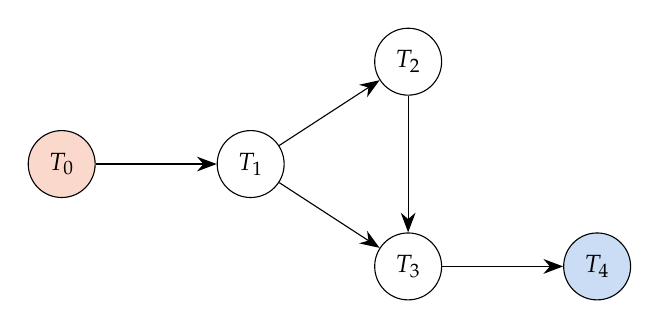
\begin{tikzpicture}[>={Stealth[length=2.5mm]}, every node/.style={circle, draw, minimum size=8.5mm, font=\small}]
  \node[fill=illicit!25] (0) at (0,0) {$T_0$};
  \node (1) at (2.4,0) {$T_1$};
  \node (2) at (4.4,1.3) {$T_2$};
  \node (3) at (4.4,-1.3) {$T_3$};
  \node[fill=licit!25] (4) at (6.8,-1.3) {$T_4$};
  \draw[->] (0) -- (1); \draw[->] (1) -- (2); \draw[->] (1) -- (3); \draw[->] (2) -- (3); \draw[->] (3) -- (4);
\end{tikzpicture}\\[2pt]
{\small $T_0$ = known illicit (label 1),\quad $T_4$ = known licit (label 0),\quad $T_1, T_2, T_3$ = unknown}
\end{center}

\textbf{Adjacency matrix, degree vector, degree matrix:}
\[
  A = \begin{bmatrix}
  0&1&0&0&0\\ 1&0&1&1&0\\ 0&1&0&1&0\\ 0&1&1&0&1\\ 0&0&0&1&0
  \end{bmatrix}, \qquad d = [1, 3, 2, 3, 1], \qquad D = \mathrm{diag}(1,3,2,3,1)
\]

\sect{B2. Add Self-Loops}
\[
  \At = A + I = \begin{bmatrix}
  1&1&0&0&0\\ 1&1&1&1&0\\ 0&1&1&1&0\\ 0&1&1&1&1\\ 0&0&0&1&1
  \end{bmatrix}
  \begin{matrix} =2\\=4\\=3\\=4\\=2 \end{matrix}
  \qquad \tilde d = [2, 4, 3, 4, 2], \quad \Dt = \mathrm{diag}(2,4,3,4,2)
\]

\sect{B3. Symmetric Normalisation}
\[
  \Dt^{-1/2} = \mathrm{diag}\Big(\tfrac{1}{\sqrt2},\ \tfrac12,\ \tfrac{1}{\sqrt3},\ \tfrac12,\ \tfrac{1}{\sqrt2}\Big),
  \qquad \Ahat_{ij} = \frac{\At_{ij}}{\sqrt{\tilde d_i \tilde d_j}}
\]
Entries: $\frac{1}{\sqrt{2\cdot2}} = \frac12$, \ $\frac{1}{\sqrt{2\cdot4}} = \frac{1}{2\sqrt2}$, \
$\frac{1}{\sqrt{4\cdot4}} = \frac14$, \ $\frac{1}{\sqrt{4\cdot3}} = \frac{1}{2\sqrt3}$, \ $\frac{1}{\sqrt{3\cdot3}} = \frac13$.
\[
  \Ahat = \begin{bmatrix}
  \frac12 & \frac{1}{2\sqrt2} & 0 & 0 & 0\\[2pt]
  \frac{1}{2\sqrt2} & \frac14 & \frac{1}{2\sqrt3} & \frac14 & 0\\[2pt]
  0 & \frac{1}{2\sqrt3} & \frac13 & \frac{1}{2\sqrt3} & 0\\[2pt]
  0 & \frac14 & \frac{1}{2\sqrt3} & \frac14 & \frac{1}{2\sqrt2}\\[2pt]
  0&0&0&\frac{1}{2\sqrt2} & \frac12
  \end{bmatrix}
  \approx
  \begin{bmatrix}
  0.5 & 0.3536 & 0 & 0 & 0\\
  0.3536 & 0.25 & 0.2887 & 0.25 & 0\\
  0 & 0.2887 & 0.3333 & 0.2887 & 0\\
  0 & 0.25 & 0.2887 & 0.25 & 0.3536\\
  0 & 0 & 0 & 0.3536 & 0.5
  \end{bmatrix}
\]
$\Ahat$ is symmetric, as required, since $\At$ is symmetric and $\Dt$ is diagonal.

\sect{B4. Feature Matrix}
Two features per transaction, $X \in \R^{5\times 2}$:
$f_1$ = ``unusual output pattern'' (1 = yes), \ $f_2$ = ``normal fee pattern'' (1 = yes).
\[
  \begin{array}{c|cc}
  \text{Tx} & f_1 & f_2 \\ \hline
  T_0 & 1 & 0\\ T_1 & 1 & 1\\ T_2 & 1 & 0\\ T_3 & 0 & 1\\ T_4 & 0 & 1
  \end{array}
  \qquad\qquad
  X = H^{(0)} = \begin{bmatrix} 1&0\\1&1\\1&0\\0&1\\0&1 \end{bmatrix}
\]

\sect{B5. Labels and Loss Weights}
$C = 2$ (class 0 = licit, class 1 = illicit). Labelled training nodes $V_L = \{T_0, T_4\}$:
\[
  y_0 = 1 \Rightarrow Y_0 = [0, 1] \ (\text{weight } 0.7), \qquad
  y_4 = 0 \Rightarrow Y_4 = [1, 0] \ (\text{weight } 0.3)
\]
$T_1, T_2, T_3$ are unlabelled during training.

\sect{B6. Layer 1: Aggregation $\bar X = \Ahat X$}
$(\Ahat X)_{ij} = \sum_k \Ahat_{ik} X_{kj}$:
\begin{align*}
  \bar X_0 &= \tfrac12(1,0) + \tfrac{1}{2\sqrt2}(1,1) = \Big(\tfrac12 + \tfrac{1}{2\sqrt2},\ \tfrac{1}{2\sqrt2}\Big) = (0.8536,\ 0.3536)\\
  \bar X_1 &= \tfrac{1}{2\sqrt2}(1,0) + \tfrac14(1,1) + \tfrac{1}{2\sqrt3}(1,0) + \tfrac14(0,1)
       = \Big(\tfrac{1}{2\sqrt2} + \tfrac14 + \tfrac{1}{2\sqrt3},\ \tfrac12\Big) = (0.8922,\ 0.5)\\
  \bar X_2 &= \tfrac{1}{2\sqrt3}(1,1) + \tfrac13(1,0) + \tfrac{1}{2\sqrt3}(0,1)
       = \Big(\tfrac{1}{2\sqrt3} + \tfrac13,\ \tfrac{1}{\sqrt3}\Big) = (0.6220,\ 0.5774)\\
  \bar X_3 &= \tfrac14(1,1) + \tfrac{1}{2\sqrt3}(1,0) + \tfrac14(0,1) + \tfrac{1}{2\sqrt2}(0,1)
       = \Big(\tfrac14 + \tfrac{1}{2\sqrt3},\ \tfrac12 + \tfrac{1}{2\sqrt2}\Big) = (0.5387,\ 0.8536)\\
  \bar X_4 &= \tfrac{1}{2\sqrt2}(0,1) + \tfrac12(0,1) = \Big(0,\ \tfrac12 + \tfrac{1}{2\sqrt2}\Big) = (0,\ 0.8536)
\end{align*}

\sect{B7. Layer 1: Transform and ReLU}
Weights (bias $= 0$ for simplicity). Hidden unit 1 = ``suspicion'' $(f_1 - f_2)$, hidden unit 2 = ``normality'' $(f_2 - f_1)$:
\[
  W^{(0)} = \begin{bmatrix} 1 & -1 \\ -1 & 1 \end{bmatrix}, \qquad
  S = \bar X\,W^{(0)} \;\Rightarrow\; S_i = \big(\bar X_{i1} - \bar X_{i2},\ \bar X_{i2} - \bar X_{i1}\big)
\]
\[
  S = \begin{bmatrix}
  0.5 & -0.5\\ 0.3922 & -0.3922\\ 0.0447 & -0.0447\\ -0.3149 & 0.3149\\ -0.8536 & 0.8536
  \end{bmatrix}
  \quad\xrightarrow{\ \mathrm{ReLU}\ }\quad
  H^{(1)} = \begin{bmatrix}
  0.5 & 0\\ 0.3922 & 0\\ 0.0447 & 0\\ 0 & 0.3149\\ 0 & 0.8536
  \end{bmatrix}
\]
ReLU sets every negative value to 0: $T_0, T_1, T_2$ activate ``suspicion''; $T_3, T_4$ activate ``normality''.

\sect{B8. Layer 2: Aggregation $M = \Ahat H^{(1)}$}
\begin{align*}
  M_0 &= \tfrac12(0.5, 0) + 0.3536(0.3922, 0) = (0.25 + 0.1387,\ 0) = (0.3887,\ 0)\\
  M_4 &= 0.3536(0, 0.3149) + \tfrac12(0, 0.8536) = (0,\ 0.1113 + 0.4268) = (0,\ 0.5381)
\end{align*}
and similarly for the other rows:
\[
  M = \Ahat H^{(1)} \approx \begin{bmatrix}
  0.3887 & 0\\ 0.2877 & 0.0787\\ 0.1281 & 0.0909\\ 0.1109 & 0.3805\\ 0 & 0.5381
  \end{bmatrix}
\]

\sect{B9. Layer 2: Output Logits $Z = M W^{(1)}$}
Suspicion should push towards illicit and normality towards licit:
\[
  W^{(1)} = \begin{bmatrix} -1 & 1 \\ 1 & -1 \end{bmatrix}
\]
With column 1 of $M$ = suspicion ($s_i$) and column 2 = normality ($n_i$):
\[
  Z_{i0} \ (\text{licit score}) = n_i - s_i, \qquad Z_{i1} \ (\text{illicit score}) = s_i - n_i = -Z_{i0}
\]
\[
  T_0: \ Z_{0} = (0 - 0.3887,\ 0.3887 - 0) = (-0.3887,\ 0.3887)
\]
All rows:
\[
  Z \approx \begin{bmatrix}
  -0.3887 & 0.3887\\ -0.2090 & 0.2090\\ -0.0372 & 0.0372\\ 0.2695 & -0.2695\\ 0.5381 & -0.5381
  \end{bmatrix}
\]

\sect{B10. Softmax}
\[
  P_{ic} = \frac{e^{Z_{ic}}}{e^{Z_{i0}} + e^{Z_{i1}}}
\]
Because $Z_{i1} = -Z_{i0}$, the two-class softmax becomes a sigmoid:
\[
  P_{i1} = \frac{e^{z}}{e^{-z} + e^{z}} = \frac{1}{1 + e^{-2z}}, \qquad z = Z_{i1}
\]
\textbf{Labelled node} $T_0$: $z = 0.3887$:
\[
  P_{0,1} = \frac{1}{1 + e^{-0.7774}} = \frac{1}{1 + 0.4596} = 0.6851, \qquad P_{0,0} = 0.3149
\]
\textbf{Labelled node} $T_4$: $z = -0.5381$:
\[
  P_{4,1} = \frac{1}{1 + e^{1.0762}} = \frac{1}{1 + 2.9335} = 0.2542, \qquad P_{4,0} = 0.7458
\]
All nodes:
\[
  P \approx \begin{bmatrix}
  0.3149 & 0.6851\\ 0.3970 & 0.6030\\ 0.4814 & 0.5186\\ 0.6316 & 0.3684\\ 0.7458 & 0.2542
  \end{bmatrix}
  \qquad
  \begin{array}{l}
  T_0: \text{illicit } \checkmark\\ T_1: \text{illicit (predicted)}\\ T_2: \text{illicit, borderline}\\ T_3: \text{licit (predicted)}\\ T_4: \text{licit } \checkmark
  \end{array}
\]
The unlabelled $T_1$ is flagged as illicit because it receives money directly from the illicit $T_0$.

\sect{B11. Weighted Cross-Entropy Loss}
\[
  \mathcal L = -\frac{w_1 \log P_{0,1} + w_0 \log P_{4,0}}{w_1 + w_0}
\]
\[
  \ell_0 = -\log(0.6851) = 0.3782, \qquad \ell_4 = -\log(0.7458) = 0.2933
\]
\[
  \mathcal L = \frac{0.7(0.3782) + 0.3(0.2933)}{0.7 + 0.3} = 0.2647 + 0.0880 = \boxed{0.3527}
\]
This is below $\ln 2 = 0.6931$, so the guess is better than random.

\sect{B12. Gradient of Softmax Cross-Entropy}
\[
  P_{ic} = \frac{e^{Z_{ic}}}{\sum_{c'} e^{Z_{ic'}}}, \qquad \ell_i = -\sum_c Y_{ic}\log P_{ic}
\]
\[
  \frac{\partial P_{ic}}{\partial Z_{ic}} = P_{ic}(1 - P_{ic}), \qquad
  \frac{\partial P_{ic}}{\partial Z_{id}} = -P_{ic}P_{id} \ (c\ne d)
\]
Combining:
\[
  \frac{\partial \ell_i}{\partial Z_{ic}} = P_{ic} - Y_{ic}
  \qquad\Rightarrow\qquad
  \frac{\partial \mathcal L}{\partial Z_i} = \frac{w_{y_i}}{\sum w}(P_i - Y_i)
\]
\begin{align*}
  T_0:&\ \ 0.7\,\big([0.3149, 0.6851] - [0, 1]\big) = [\,0.2204,\ -0.2204\,]\\
  T_4:&\ \ 0.3\,\big([0.7458, 0.2542] - [1, 0]\big) = [\,-0.0763,\ 0.0763\,]
\end{align*}
\[
  dZ = \begin{bmatrix} 0.2204 & -0.2204\\ 0&0\\ 0&0\\ 0&0\\ -0.0763 & 0.0763 \end{bmatrix}
  \qquad (\text{unlabelled rows are } 0)
\]

\sect{B13. Backpropagation to $W^{(1)}$}
Since $Z = M W^{(1)}$:
\[
  \frac{\partial\mathcal L}{\partial W^{(1)}} = M^T dZ = M_0^T dZ_0 + M_4^T dZ_4
\]
\[
  = \begin{bmatrix} 0.3887\\0 \end{bmatrix}[0.2204,\ -0.2204] + \begin{bmatrix} 0\\0.5381 \end{bmatrix}[-0.0763,\ 0.0763]
  = \begin{bmatrix} 0.0857 & -0.0857\\ -0.0410 & 0.0410 \end{bmatrix}
\]

\sect{B14. Backpropagation to $H^{(1)}$}
\[
  dM = dZ\, W^{(1)T}: \quad dM_0 = [-0.4408,\ 0.4408], \quad dM_4 = [0.1525,\ -0.1525], \quad \text{others } 0
\]
Since $M = \Ahat H^{(1)}$ and $\Ahat^T = \Ahat$:
\[
  dH^{(1)} = \Ahat\, dM \;\Rightarrow\; dH_i = \Ahat_{i0}\, dM_0 + \Ahat_{i4}\, dM_4
\]
\[
  dH^{(1)} = \begin{bmatrix}
  -0.2204 & 0.2204\\ -0.1559 & 0.1559\\ 0 & 0\\ 0.0539 & -0.0539\\ 0.0763 & -0.0763
  \end{bmatrix}
\]
$T_1$ and $T_3$ get a gradient even though they are unlabelled, because they are neighbours of $T_0$ and $T_4$.

\sect{B15. Through ReLU and to $W^{(0)}$}
ReLU passes the gradient only where $S > 0$:
\[
  dS = dH^{(1)} \odot \mathbb 1[S > 0] = \begin{bmatrix}
  -0.2204 & 0\\ -0.1559 & 0\\ 0 & 0\\ 0 & -0.0539\\ 0 & -0.0763
  \end{bmatrix}
\]
\[
  \frac{\partial\mathcal L}{\partial W^{(0)}} = (\Ahat X)^T dS = \bar X^T dS
\]
\begin{align*}
  [1,1]:&\ \ 0.8536(-0.2204) + 0.8922(-0.1559) = -0.3272\\
  [1,2]:&\ \ 0.5387(-0.0539) = -0.0291\\
  [2,1]:&\ \ 0.3536(-0.2204) + 0.5(-0.1559) = -0.1559\\
  [2,2]:&\ \ 0.8536(-0.0539) + 0.8536(-0.0763) = -0.1111
\end{align*}
\[
  \frac{\partial\mathcal L}{\partial W^{(0)}} = \begin{bmatrix} -0.3272 & -0.0291\\ -0.1559 & -0.1111 \end{bmatrix}
\]

\sect{B16. Gradient Descent Update ($\eta = 0.5$)}
\[
  W \leftarrow W - \eta\, \frac{\partial \mathcal L}{\partial W}
\]
\[
  W^{(0)}_{\text{new}} = \begin{bmatrix} 1 & -1\\ -1 & 1 \end{bmatrix} - 0.5\begin{bmatrix} -0.3272 & -0.0291\\ -0.1559 & -0.1111 \end{bmatrix}
  = \begin{bmatrix} 1.1636 & -0.9855\\ -0.9221 & 1.0556 \end{bmatrix}
\]
\[
  W^{(1)}_{\text{new}} = \begin{bmatrix} -1 & 1\\ 1 & -1 \end{bmatrix} - 0.5\begin{bmatrix} 0.0857 & -0.0857\\ -0.0410 & 0.0410 \end{bmatrix}
  = \begin{bmatrix} -1.0428 & 1.0428\\ 1.0205 & -1.0205 \end{bmatrix}
\]
Repeating the forward pass with the new weights:
\[
  P_{0,1}: 0.6851 \rightarrow 0.7542, \qquad P_{4,0}: 0.7458 \rightarrow 0.7661, \qquad
  \mathcal L: 0.3527 \rightarrow \boxed{0.2773}
\]
The loss decreased, so one full training iteration of the vanilla GCN is complete. The real model repeats this
200 times with Adam on 203,769 transactions.

\sect{B17. Over-smoothing on the Small Graph}
Apply $\Ahat$ repeatedly with no weights, $H_k = \Ahat^k X$, and measure the mean cosine similarity between all pairs of rows:
\begin{center}
\begin{tabular}{lcccccc}
\toprule
$k$ & 1 & 2 & 4 & 8 & 16 & 32 \\
\midrule
mean cosine similarity & 0.7962 & 0.8922 & 0.9739 & 0.9987 & 1.0000 & 1.0000 \\
\bottomrule
\end{tabular}
\end{center}
Eigenvalues of $\Ahat$: \ $1,\ 0.6830,\ 0.4302,\ -0.0969,\ -0.1830$.

Top eigenvector:
\[
  \pi \propto \sqrt{\tilde d} = [\sqrt2, 2, \sqrt3, 2, \sqrt2] \;\Rightarrow\; \pi = [0.3651,\ 0.5164,\ 0.4472,\ 0.5164,\ 0.3651]
\]

Limit: $H_\infty = \pi\pi^T X$, with $\pi^T X = [1.3287,\ 1.3979]$:
\[
  H_\infty = \begin{bmatrix}
  0.485 & 0.510\\ 0.686 & 0.722\\ 0.594 & 0.625\\ 0.686 & 0.722\\ 0.485 & 0.510
  \end{bmatrix}
\]
Every row is a multiple of $[1.3287, 1.3979]$. The illicit $T_0$ and the licit $T_4$ now have \emph{identical} features,
so they cannot be told apart. This is why we use only 2 layers.

\end{document}
